\section{Scenario 1}\label{sec:scenario1}
Curvature Scenario

\begin{figure}[H]
\hfill
\subfigure[.]{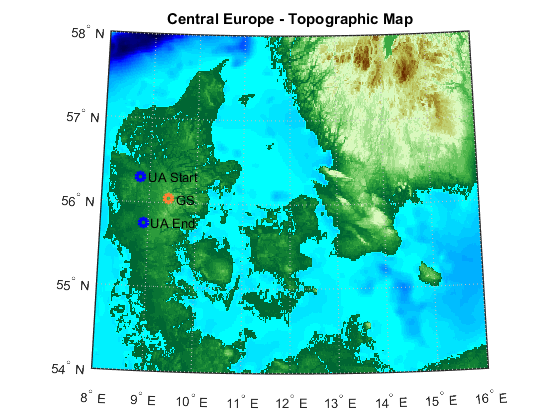
\includegraphics[scale=0.45]{figures/s1_topographic_map.png}}
\hfill
\subfigure[caption]{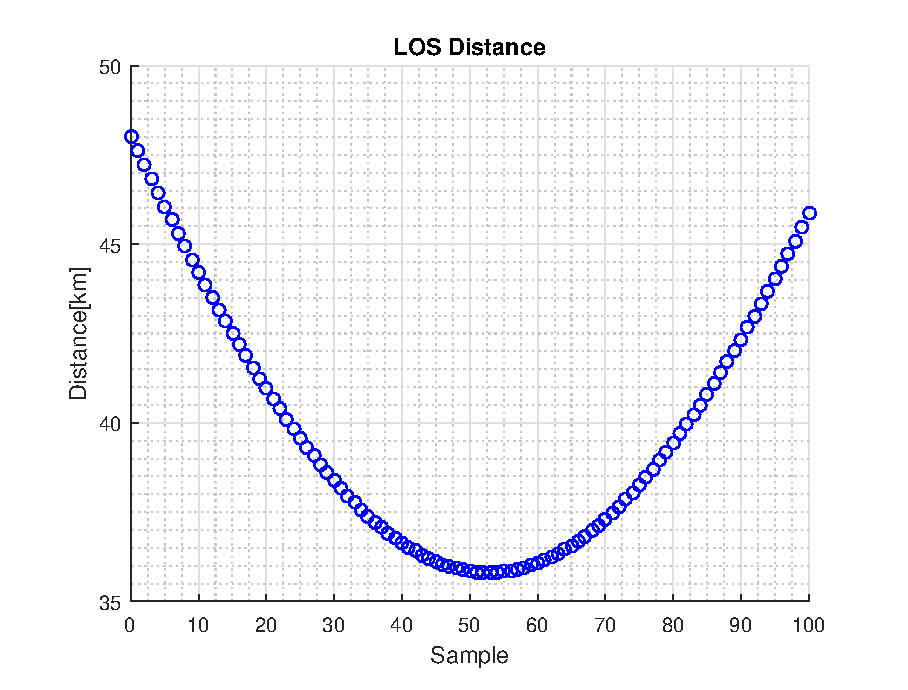
\includegraphics[scale=0.45]{figures/s1_los_distance.eps}}
\hfill
\caption{caption}
\label{fig:topigraphic}
\end{figure}

\subsection{Drones}

Figure \ref{fig:s1_drones_p}, \ref{fig:s1_drones_pi}, \ref{fig:s1_drones_pd} and \ref{fig:s1_drones_pid}.
\begin{figure}[H]
\begin{minipage}[t]{0.45\textwidth}
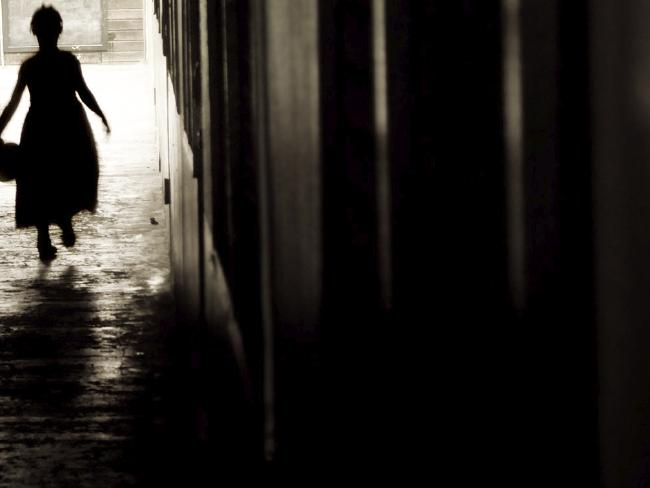
\includegraphics[width=\linewidth]{figures/randomfigure.jpg}
\caption{p}
\label{fig:s1_drones_p}
\end{minipage}
\hspace{\fill}
\begin{minipage}[t]{0.45\textwidth}
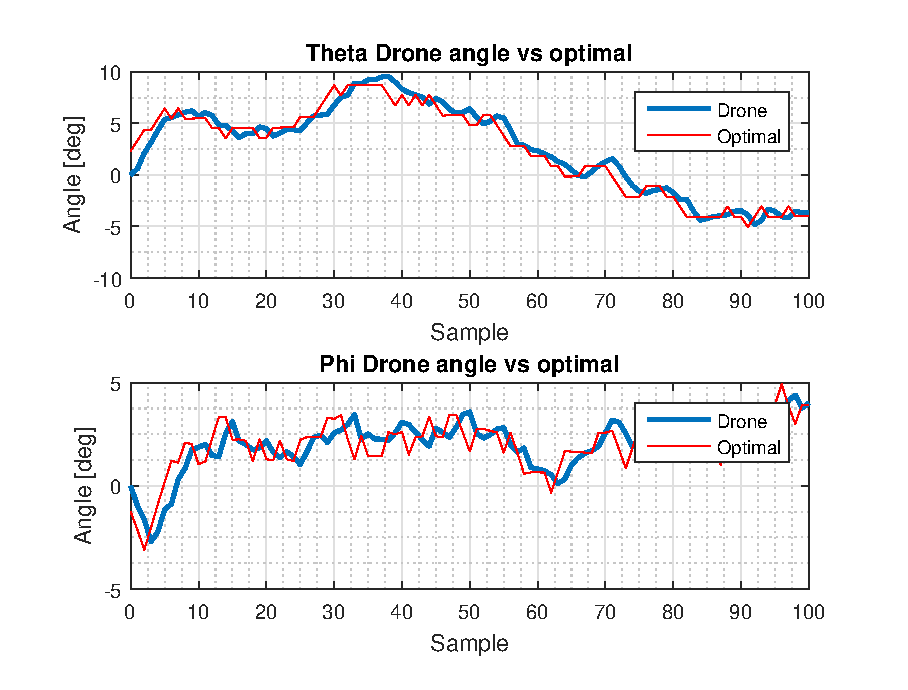
\includegraphics[width=\linewidth]{figures/s2_pi_drone_theta_phi_optimal.eps}
\caption{pi}
\label{fig:s1_drones_pi}
\end{minipage}

\vspace*{0.5cm} % (or whatever vertical separation you prefer)
\begin{minipage}[t]{0.45\textwidth}
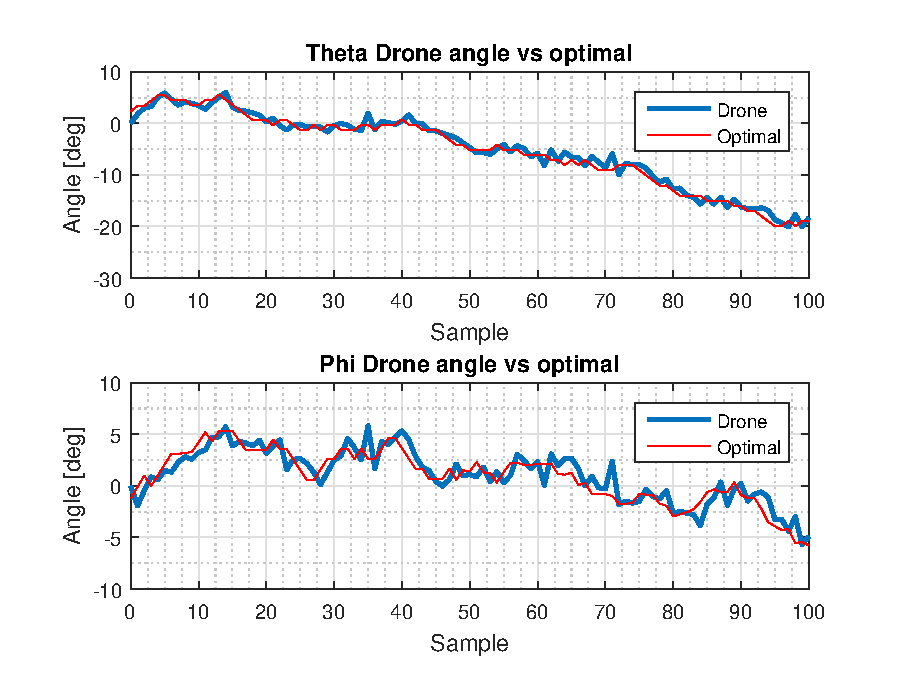
\includegraphics[width=\linewidth]{figures/s2_pd_drone_theta_phi_optimal.eps}
\caption{pd}
\label{fig:s1_drones_pd}
\end{minipage}
\hspace{\fill}
\begin{minipage}[t]{0.45\textwidth}
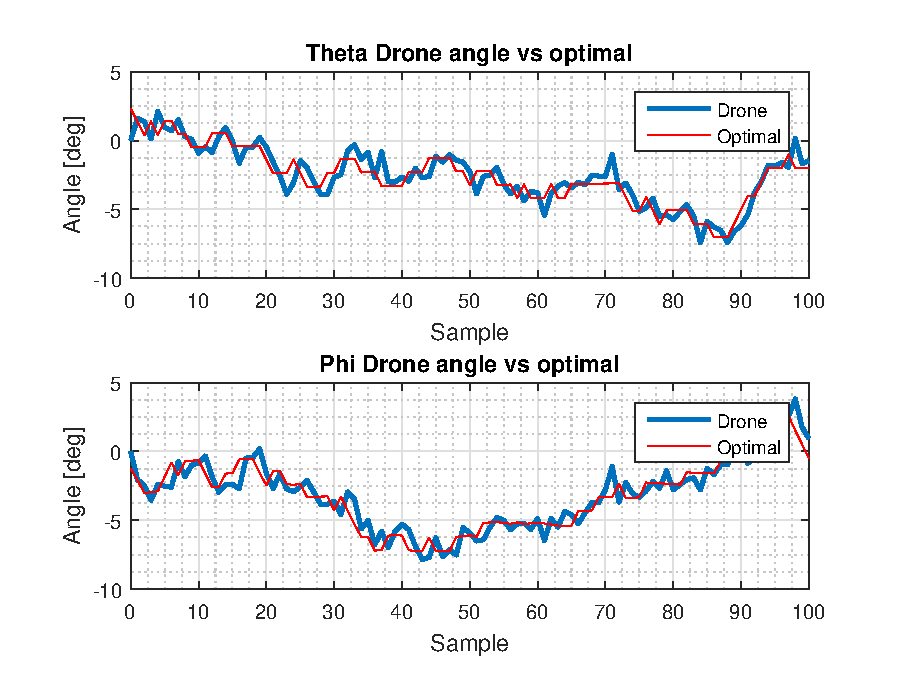
\includegraphics[width=\linewidth]{figures/s2_pid_drone_theta_phi_optimal.eps}
\caption{pid}
\label{fig:s1_drones_pid}
\end{minipage}

\end{figure}
